\chapter{Suitability of Tracks as Fake Proxies}
\label{app:MOSSFlepton,track}

We look at the invariant mass of opposite-sign muon + track pairs. If the tracks are uncorrelated with the muons, we expect a broad peak at the average invariant mass. If they are correlated, they will be related to their source, for example a \Z decay. In fact, we see both (Figure~\ref{fig:app:MOSSFlepton,track}).

\begin{sidewaysfigure}
\begin{center}
	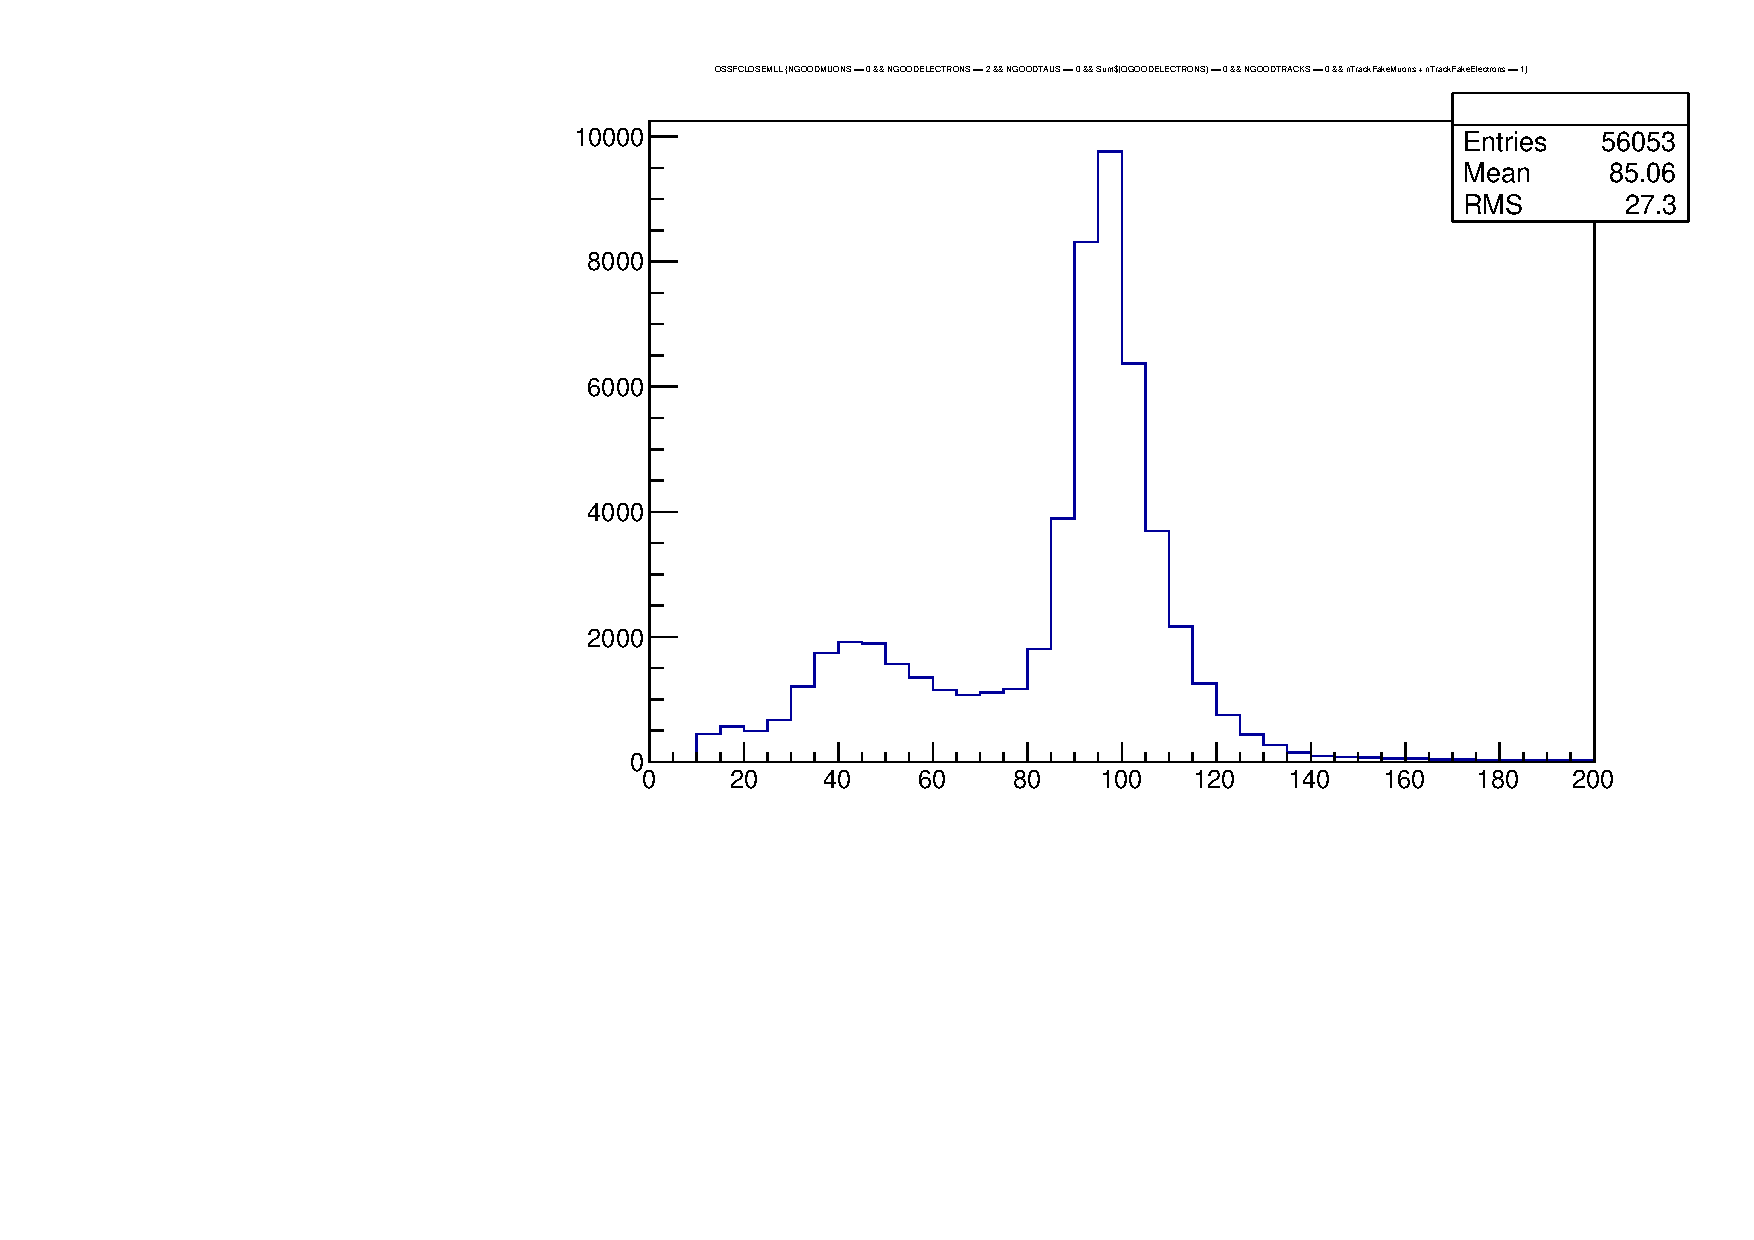
\includegraphics[width=.5\textwidth]{Appendix/study_OSSFCLOSEMLL_electron,track_dileptons-1fake}%
	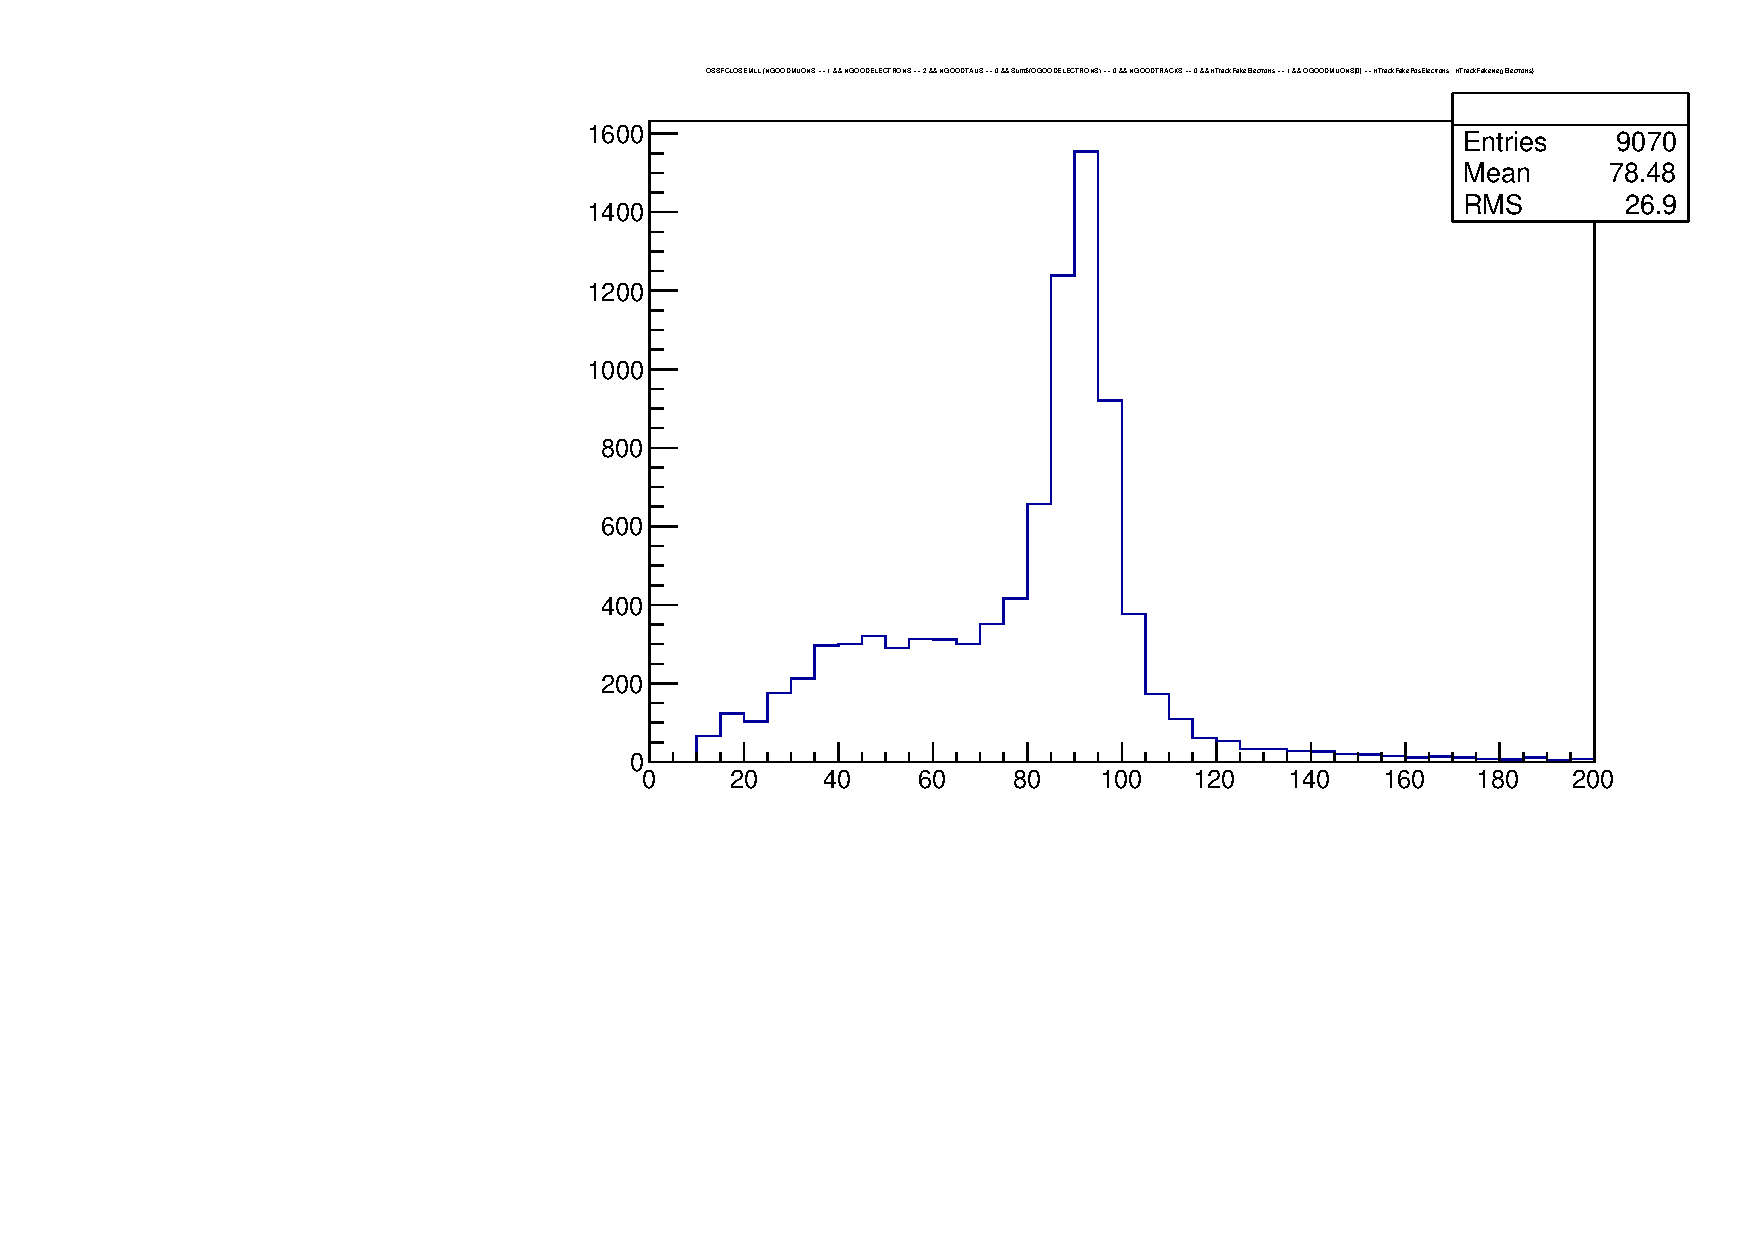
\includegraphics[width=.5\textwidth]{Appendix/study_OSSFCLOSEMLL_electron,track_1fake}\\
	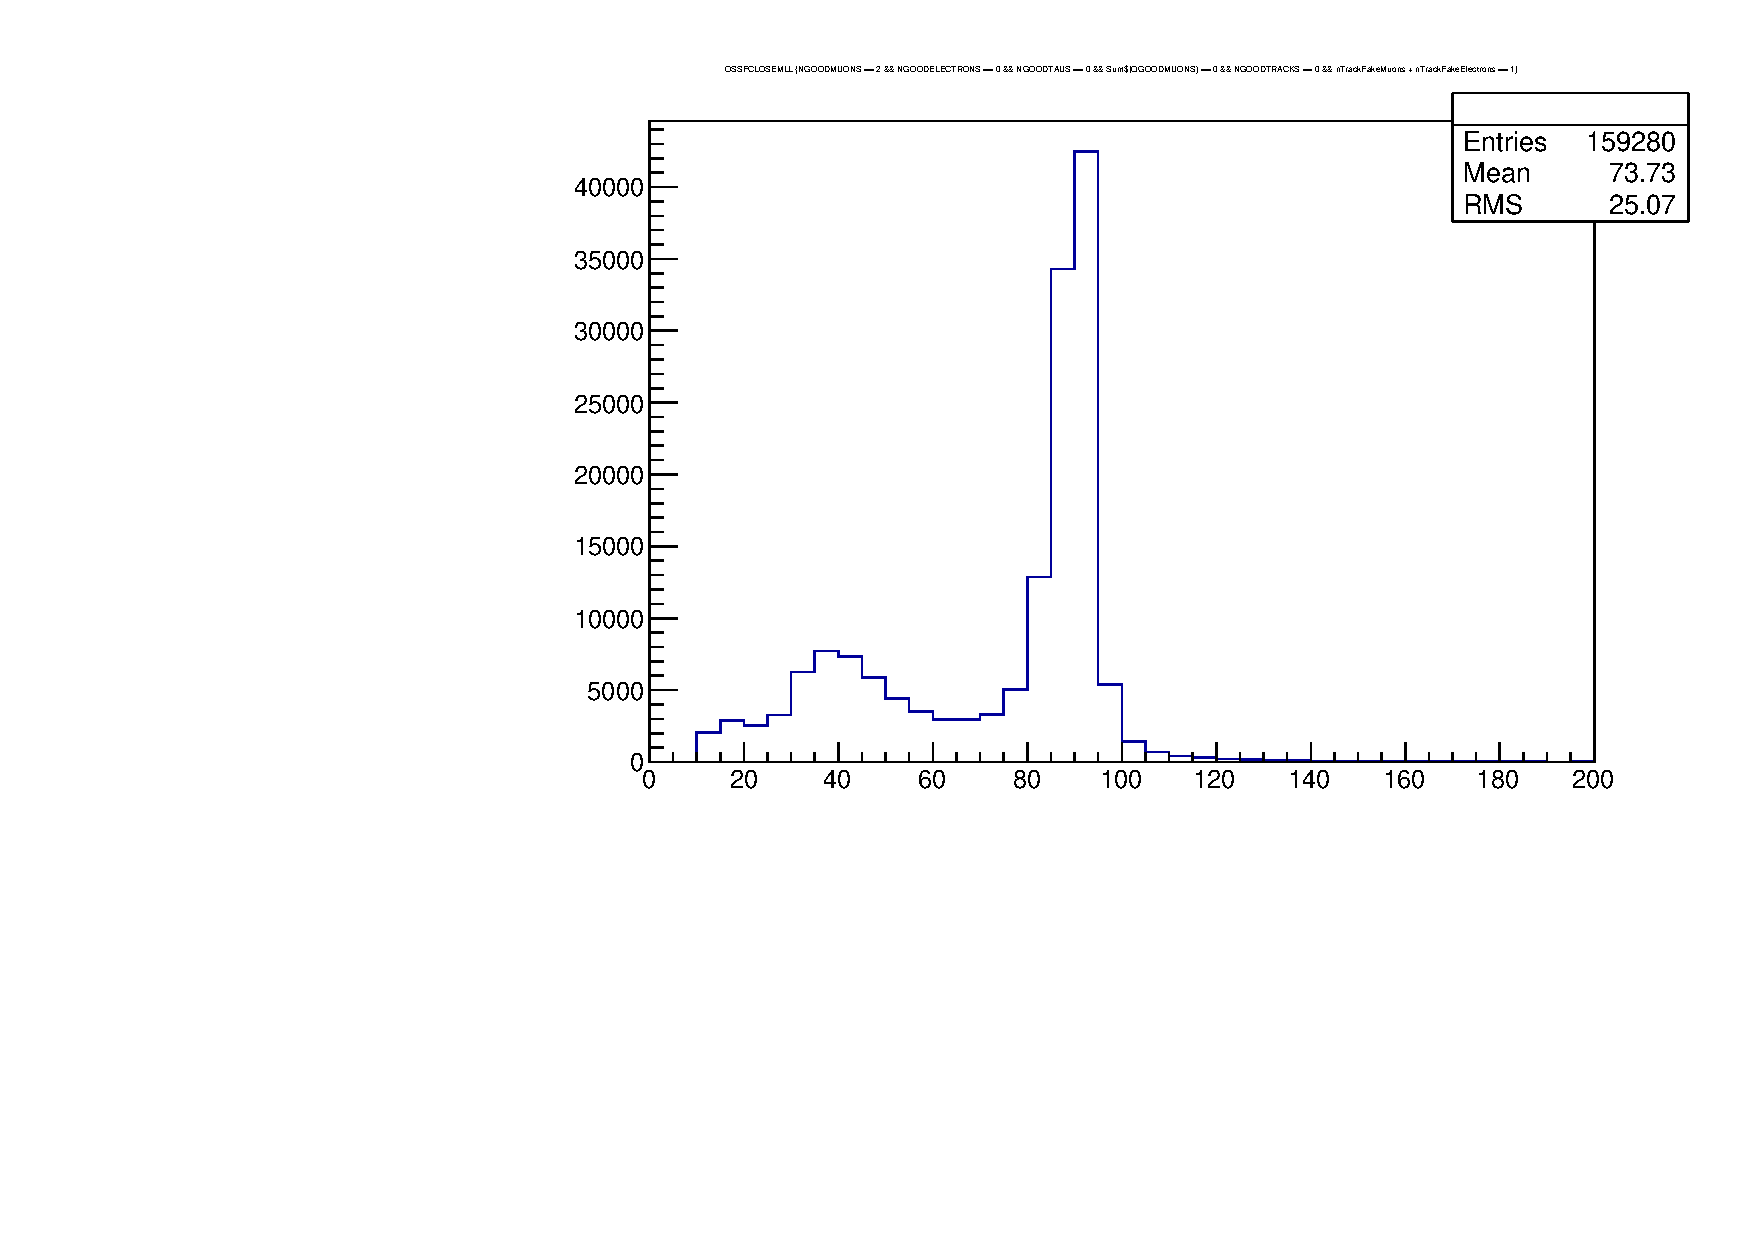
\includegraphics[width=.5\textwidth]{Appendix/study_OSSFCLOSEMLL_muon,track_dileptons-1fake}%
	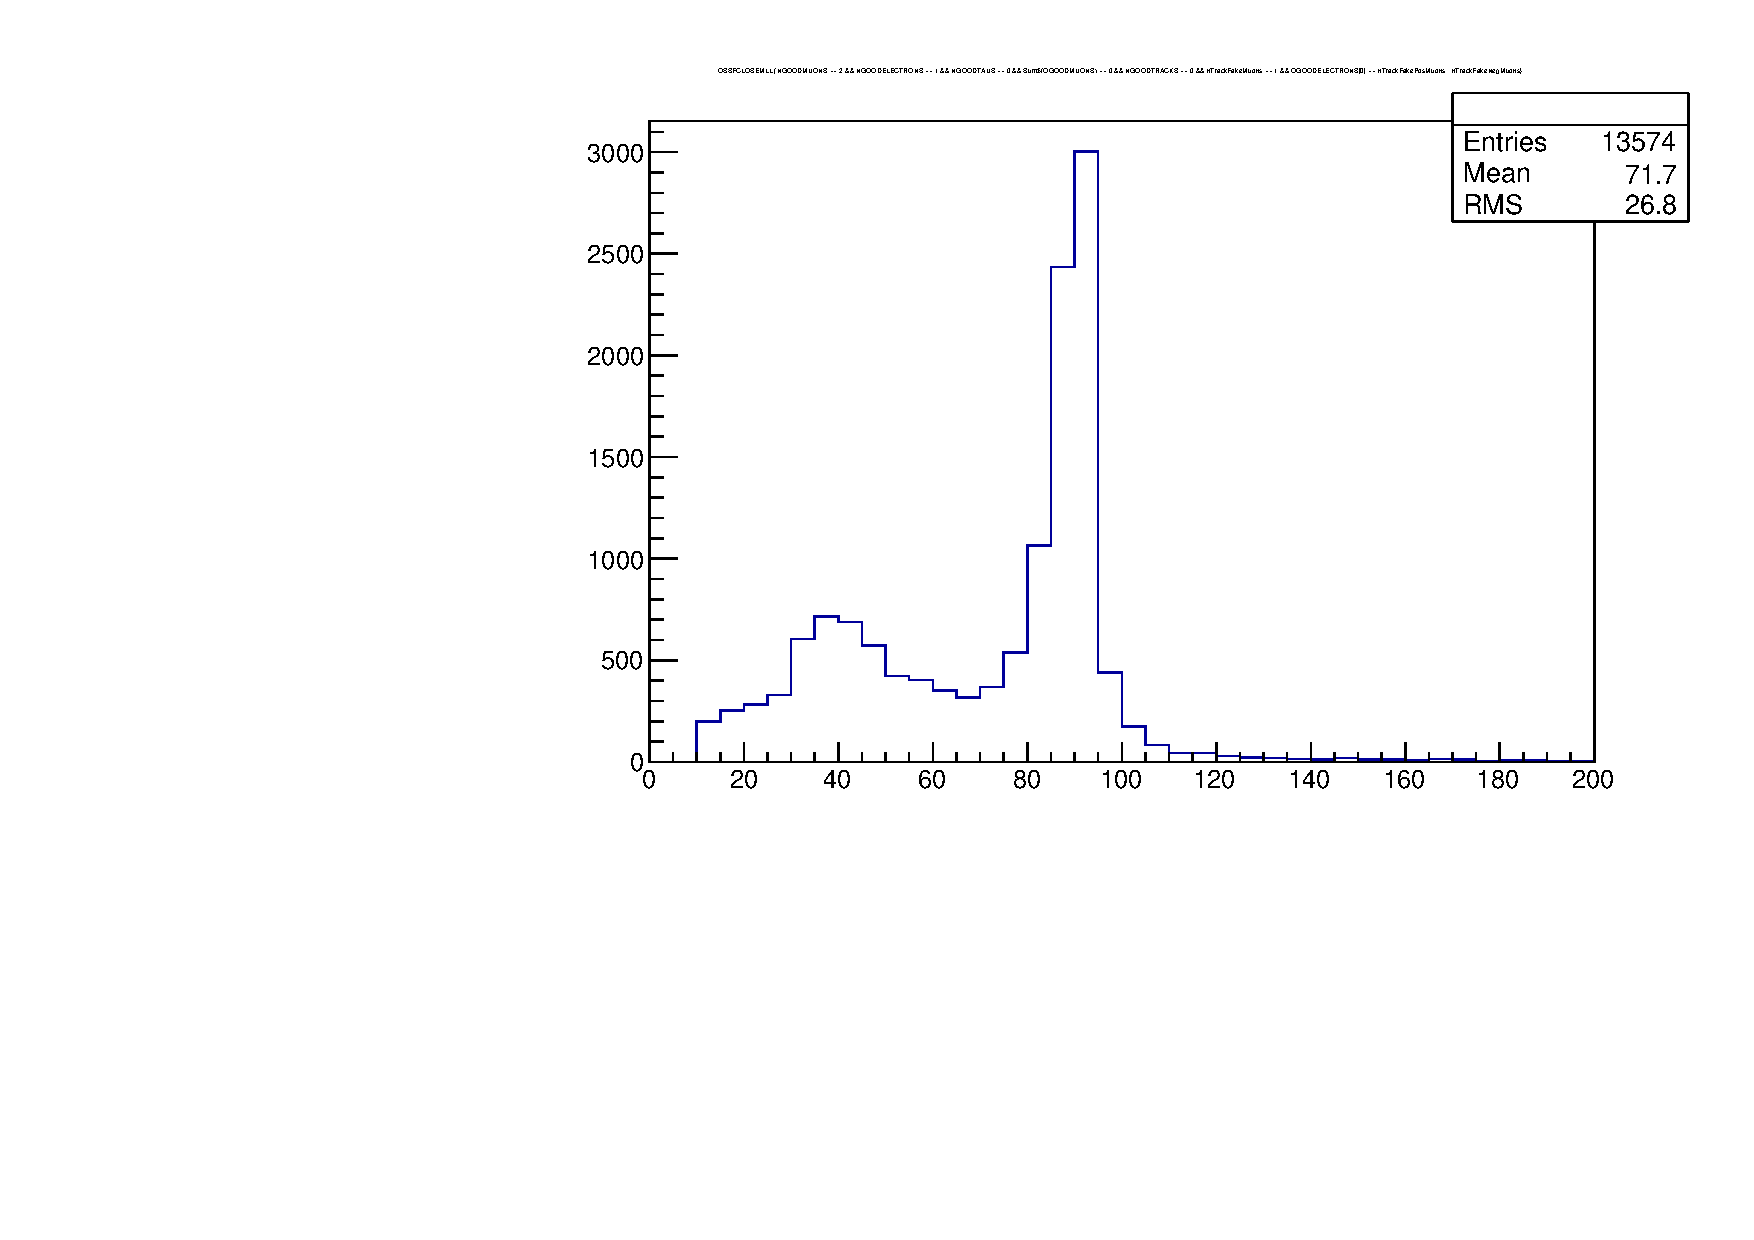
\includegraphics[width=.5\textwidth]{Appendix/study_OSSFCLOSEMLL_muon,track_1fake}
	\caption{Top: $m_{et}$ distribution; bottom: $m_{\mu t}$ distribution. Left: no other leptons present, right: additional lepton present. If a third lepton is present, its flavor is opposite of the first lepton, and its charge is the same as the track's (rejecting third leptons from \Z).\\
	\textbf{Note:} This is from the dilepton-triggered dataset, i.e. the tracks used here probably were good enough leptons to trigger.
	\label{fig:app:MOSSFlepton,track}}
\end{center}
\end{sidewaysfigure}

This suggests that tracks are not only from jets, but also from low quality leptons. So, tracks do model fake leptons from jets, and at the same time also model leptons that were vetoed by quality cuts. However, since both effects also occur in the signal regions, the overall shape of the track background is still expected to be accurate there.

Note that the numbers in Fig.~\ref{fig:app:MOSSFlepton,track} have been derived with the 8\TeV CMS dataset from Run I. The conclusions, however, are also valid for Run II at 13\TeV.
